\section{Versuchsaufbau und -durchführung} \label{sec:aufbau}

	In diesem Abschnitt werden der Aufbau und die Durchführung des Versuchs behandelt.

\subsection*{Aufbau}
	
%	\begin{figure}[h]
%		\centering
%		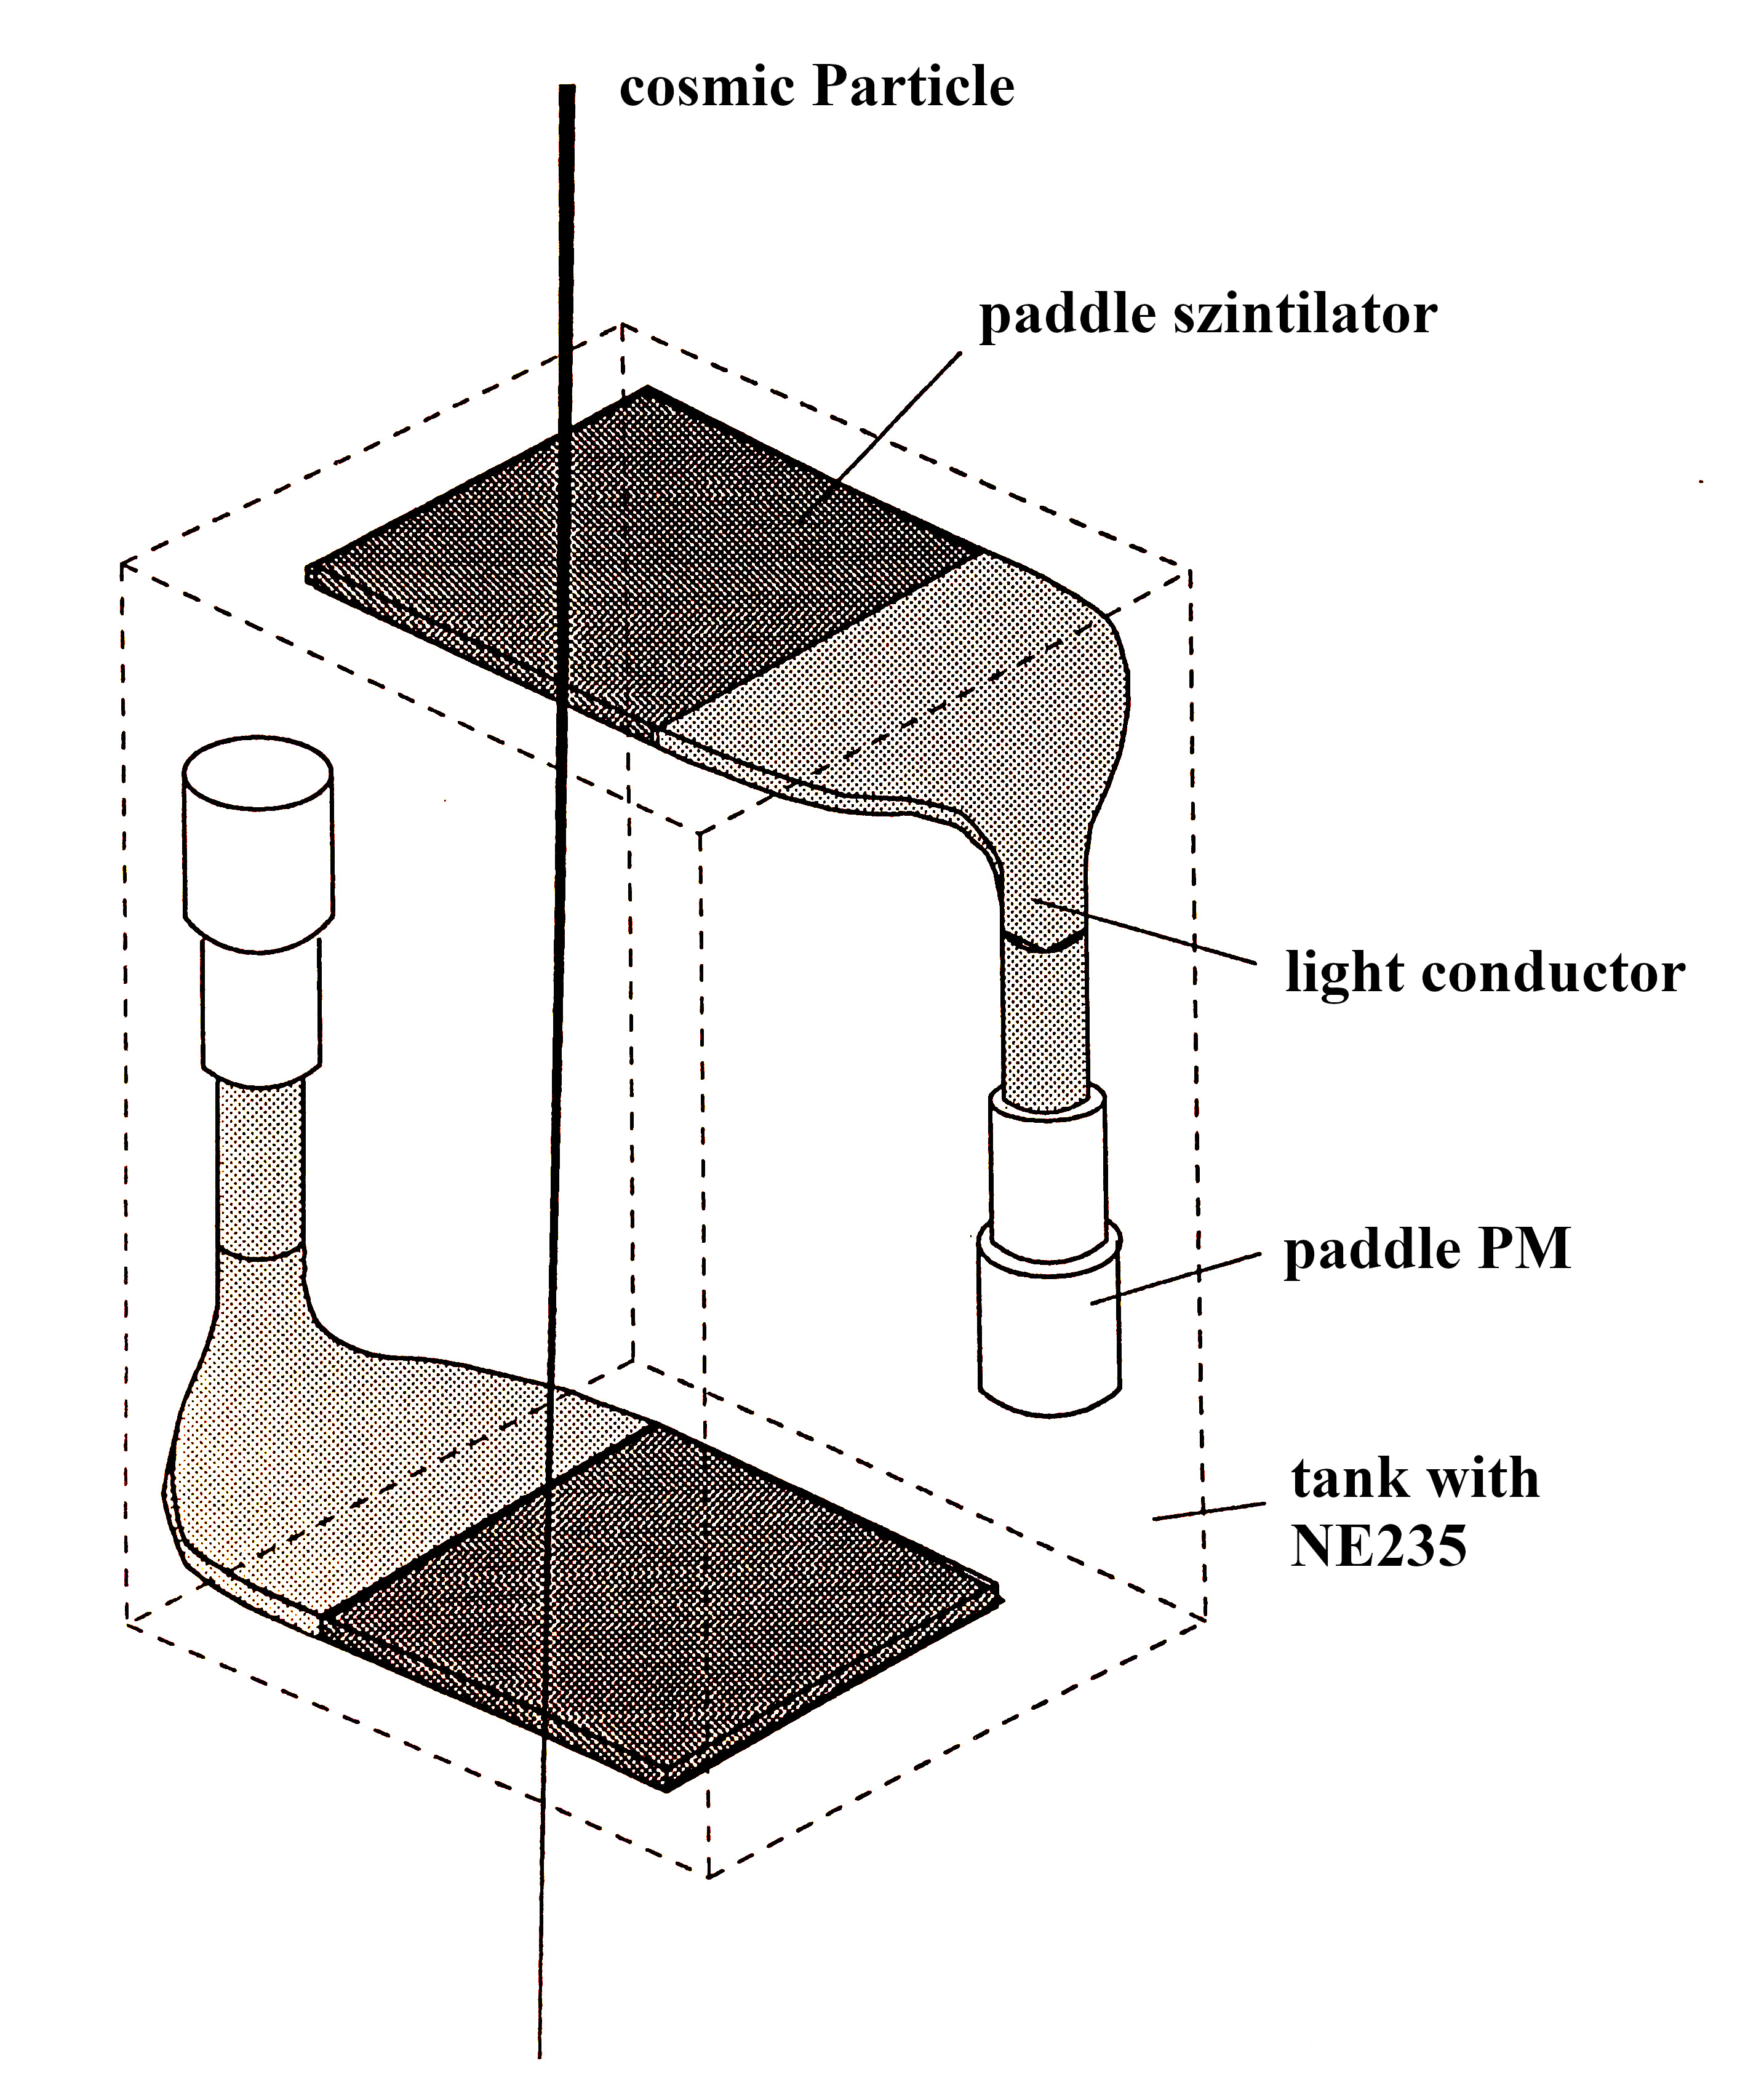
\includegraphics[width=.8\textwidth]{img/aufbau.png}
%		\caption{Skizze des Versuchsaufbau.\cite{wwu}}
%		\label{fig:aufbau}
%	\end{figure}

	\begin{figure}[H]
		\centering
		\begin{subfigure}[c]{\textwidth}		
			\centering	
			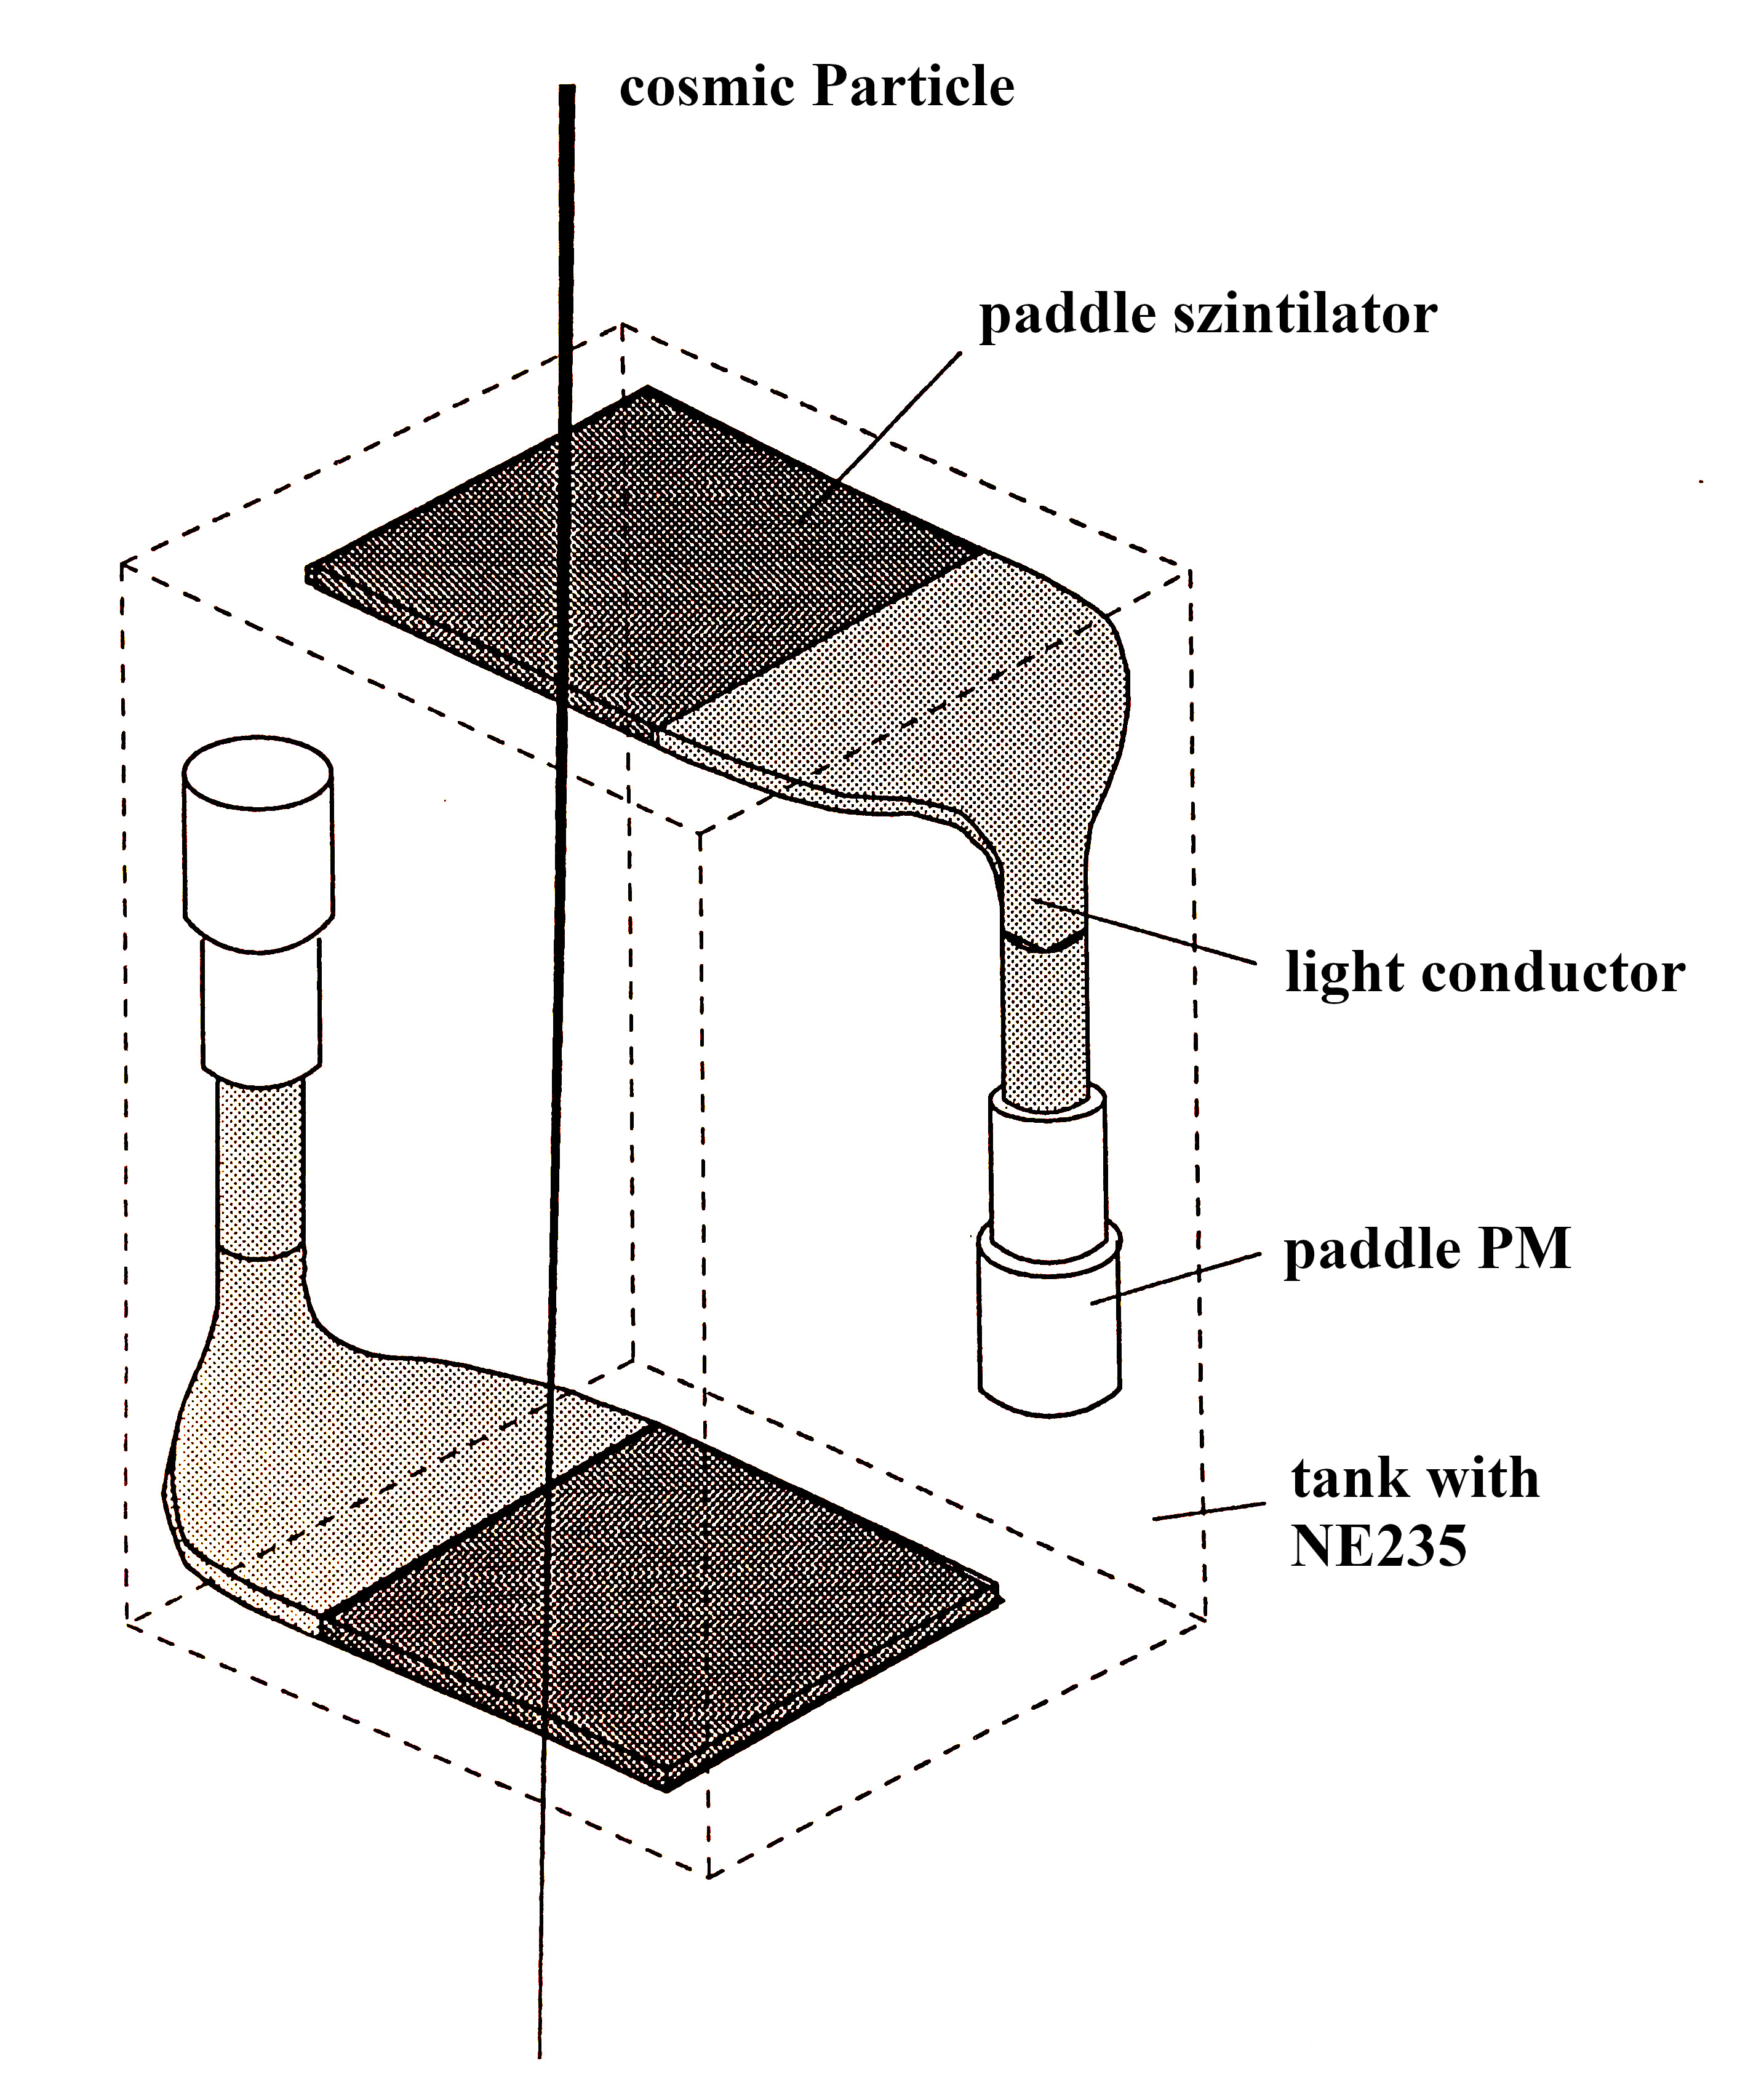
\includegraphics[width=0.7\textwidth]{img/aufbau.png}
		\end{subfigure}
		
		\begin{subfigure}[c]{\textwidth}
			\centering
			\includegraphics[width=0.7\textwidth]{img/aufbau2.png}
		\end{subfigure}
		
		\caption{Skizze des Versuchaufbaus. 
			Oben zur Messung der einzelnen Komponenten. 
			Unten zur Untersuchung der Eigenschaften von Koaxialkabeln. \cite{wwu}}
		\label{fig:aufbau}
	\end{figure}

	Der Versuch wird wie in \cref{fig:aufbau} dargestellt aufgebaut.
	Zu erkennen sind ein Mikrowellengenerator, das zu vermessende Objekt, die Messdiode und ein Multimeter.
	Bei der Vermessung einzelner Bauteile werden diese direkt zwischen Diode und Mikrowellengenerator geschaltet.
	Um hingegen die Koaxialkabel zu untersuchen, muss das Signal zunächst über einen Zirkulator umgelenkt werden.
	Sowohl Mikrowellengenerator als auch Multimeter sind mit einem Computer verbunden, auf dem die LabVIEW-Programme "Messungen Frequenz" und "Messungen Leistung" zur Aufnahme der Daten vorliegen.
	Verbunden werden Mikrowellengenerator und Multimeter über Koaxialkabel mit Messobjekt und Diode.
	Die Verbindung zu dem Computer erfolgt über GPIB-Kabel.
	Alle nicht verwendeten Anschlüsse werden mit einem angepassten Abschlusswiderstand von \SI{50}{\ohm} versehen, um Reflexionen und somit ungewollte Interferenzerscheinungen zu verhindern.
	
	Für die Messung werden das Digitalmultimeter TTi 1906 und der Mikrowellengenerator Wiltron 6759B verwendet.
	Bei der Diode handelt es sich um eine Schottky-Diode.
	
\subsection*{Durchführung}

	Angefangen wird mit der Messung der Kennlinie der Diode.
	Da sie Bestandteil aller Messungen ist, dient sie als Referenz.
	Hierzu wird kein Messobjekt angeschlossen und das LabVIEW-Programm "Messungen Leistung" verwendet.
	Gemessen wird die Spannung am Multimeter in Abhängigkeit von der Eingangsleistung am Mikrowellengenerator.
	Dabei wird ein Leistungsbereich von \SIrange{-20}{15}{\decibelmilliwatt} gewählt, eine Messpunktzahl von 71 und eine Frequenz von \SI{5}{\giga\hertz} für die elektromagnetische Welle.
	
	\
	
	Die weiteren Messungen erfolgen nach einem ähnlichem Schema.
	Hier wird nun die Leistung bei \SI{10}{\decibelmilliwatt} festgehalten und die Frequenz über das LabVIEW-Programm "Messungen Frequenz" variiert und weiterhin die Spannung an dem Multimeter gemessen.
	Die Frequenzbereiche werden anhand der vorliegenden Bauteilinformationen so gewählt, dass sie den gesamten Bereich abdecken für den sie vorgesehen sind.
	
	Zunächst wird der Richtleiter vermessen.
	Dazu werden über die Torpaare (1-2), (1-4) und (2,4) gemessen, sodass daraus im nächsten Abschnitt die unterschiedlichen Kenngrößen ermittelt werden können.
	
	Als nächstes werden zwei Zirkulatoren vermessen, jeweils einmal in Durchlass- (1-2) und Sperrrichtung (2-1).
	Da es sich um symmetrische Bauteile handelt, wird nicht über gleichwertige Torpaare wie (2-3) gemessen.
	Genau gleich (abgesehen von den Bauteilparametern) verläuft die Messung des Isolators.
	
	Zuletzt wird einer der beiden Zirkulatoren erneut in Durchlassrichtung angeschlossen.
	An dieser Stelle befindet sich jedoch nicht die Diode an Tor 2 sondern ein kapazitives Koppelstück, welches mit einem Koaxialkabel verbunden ist.
	Das Ende des Kabels wird mit einem Abschlusswiderstand kurzgeschlossen.
	Tor 3 wird nun mit der Diode verbunden, von der das Signal wie zuvor zum Multimeter führt.
	Durchgeführt wird die Messung für zwei Koaxialkabel unterschiedlicher Länge wie zuvor, jedoch bei einer festen Leistung von \SI{5}{\decibelmilliwatt}.
	